\section{Muon combinatorial background}

Two unrelated muons in time that form a vertex pointing to the target.

\begin{table}[h]
\centering\small
\caption{\texttt{D6\_straw\_mod}, per 15 years. \src{docs/STATUS.md (2026-11-09, 2026-11-10 night)}}
\begin{tabular}{@{}lrrrl@{}}
\toprule
Inputs & candidates & IP $<10$\,cm & after veto & note\\
\midrule
dataset c (\texttt{inputs\_c\_s}), $\mu\times\mu$ & 852 & 405 & 51 & legs explained 0.74 / 0.64\\
dataset c, $\mu\times$rock & 8\,190 & 2\,927 & 0.023 & rock leg explained 0.9999\\
dataset c, rock$\times$rock & $5\times10^{-7}$ & 0 & 0 & \\
Nov-4 (\texttt{inputs\_nov4}), $\mu\times\mu$ & 2.86 & -- & 0.014 & 0.003 with EM debris\\
\bottomrule
\end{tabular}
\end{table}

\begin{itemize}
\item The $\times140$ difference between dataset c and Nov-4 is \textbf{not the layout}: dataset c has 3--4$\times$ more
SST1 muons at 30--100\,GeV near the axis (source pool, D5), the pair rate goes as the square, times the pointing
preference, times the old $5\times10^{13}$ normalisation of \texttt{inputs\_c\_s}. \open: compare pool v2/v3 and Nov-4
spectra above 100\,GeV by component.
\item On the factorised estimate (A1): closure on \texttt{inputs.npz} D0\_minimal 1\,694 observed vs 1\,702 factorised
($p=0.86$); for vetoed designs 0 observed, $<7.6\times10^{-4}$ (90\,\% CL). \src{ISSUES.txt A1}
\item Source systematic (D5): the enriched tail's angles raise the SST1-selected rate by $\times1.55$ (convention
$\times0.905$, tail angles $\times0.56$); kept as is, quoted as $+40\,\%$ on the SST1-selected rate.
\end{itemize}

\begin{figure}[h]
\centering
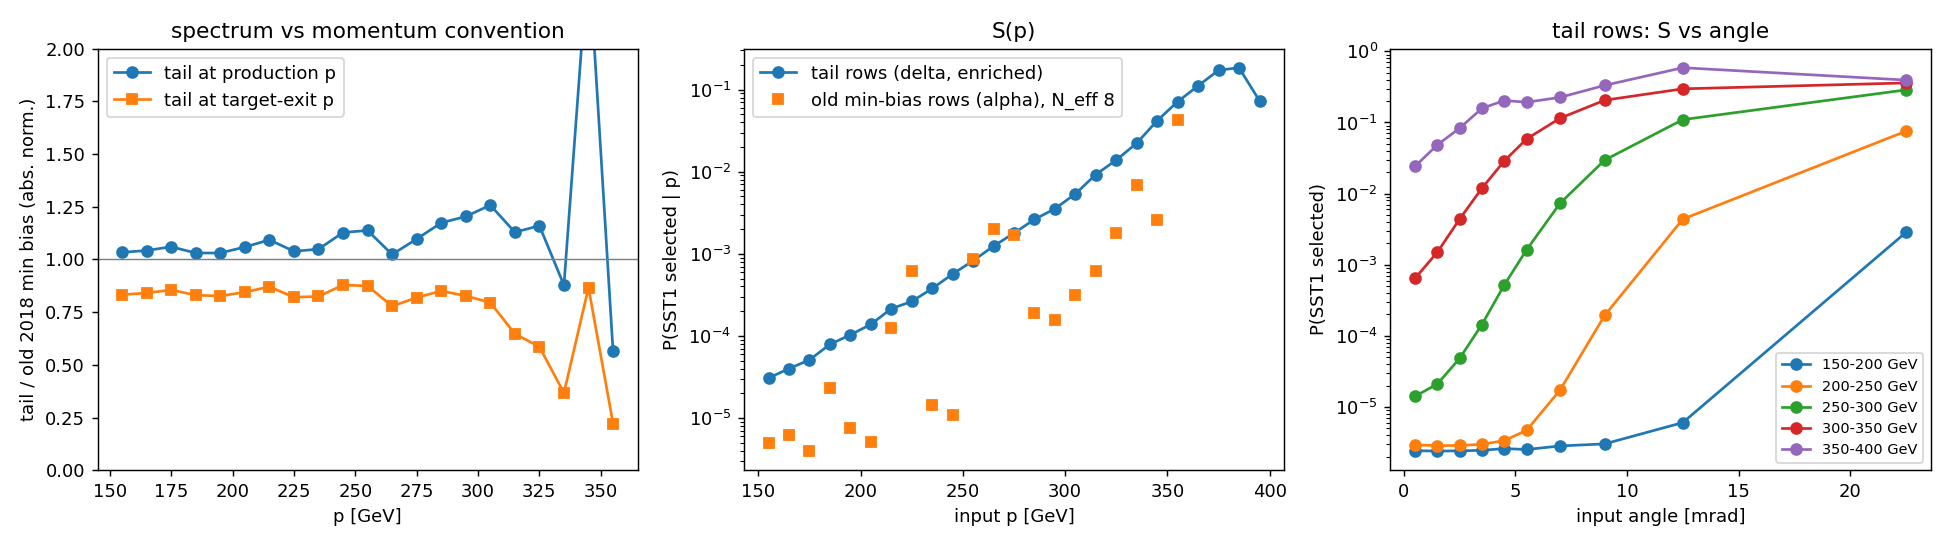
\includegraphics[width=0.95\linewidth]{d5_summary.png}
\caption{D5 check: momentum convention and tail angles of the enriched source. \src{results/d5_convention/d5_summary.png}}
\end{figure}
